% !TeX spellcheck = en_GB
% ***************************************************** %
\section{Introduction}\label{sc:intro}
% ***************************************************** %

% problem identification
% solutions

\subsection{Classification task}

\subsection{Optimization problem}

\[
\min_{w\in\R^p}\func(w)=L(w)+\lambda\Omega(w)
\]

%\[
%\func(w)=\sum_{i=1}^Nf_i(w)+\lambda\norma{w}^2
%\]

\begin{equation}\label{eq:opt-prob}
\min\frac{1}{N}\sum_{i=1}^N\log\bigl(1+\exp(-y^{(i)}w^Tx^{(i)})\bigr)+\lambda\norma{w}^2
\end{equation}
where $i=\,\dots,N$ are the dataset indices, $y^{i}\in\set{-1,1}$ is the response variable corresponding to the negative or positive class, $x^{i}\in\R^p$ are dataset examples.

\[
\nabla\func(w)=\frac{1}{N}X^Tr+2\lambda w,\quad r_i=-y^{(i)}\sigma(-y^{(i)}w^Tx^{(i)})
\]

\[
\nabla^2\func(w)=\frac{1}{N}XDX^T+2\lambda I,\quad d_{ii}=\sigma(y^{(i)}w^Tx^{(i)})\sigma(-y^{(i)}w^Tx^{(i)})
\]
$r\in\R^N$, $D\in\R^{N\times N}$

\begin{prop}
Problem~\eqref{eq:opt-prob} admits a unique optimal solution.
\end{prop}

\[
X^T=
\begin{pmatrix}
1 & x_1^{(1)} & x_2^{(1)} & \dots & x_p^{(1)} \\
1 & x_1^{(2)} & x_2^{(2)} & \dots & x_p^{(2)} \\
\vdots & \vdots & \vdots & \ddots & \vdots \\
1 & x_1^{(N)} & x_2^{(N)} & \dots & x_p^{(N)}
\end{pmatrix}\in\R^{N\times(p+1)}
\]

\[
w=
\begin{pmatrix}
b \\ w_1 \\ w_2 \\ \vdots \\ w_p
\end{pmatrix}\in\R^{(p+1)}
\]

\[
y=
\begin{pmatrix}
y^{(1)} \\ y^{(2)} \\ \vdots \\ y^{(N)}
\end{pmatrix}\in\set{-1,1}
\]

\[
x^{(i)}=
\begin{pmatrix}
1 \\ x_1^{(i)} \\ x_2^{(i)} \\ \vdots \\ x_N^{(i)}
\end{pmatrix}\in\R^{(p+1)}
\]

\cleardoublepage

%\begin{figure}
%\centering
%\begin{tikzpicture}
%\begin{axis}[xlabel=$uv$,ylabel=$\ell$]
%\addplot[samples=200,blue,smooth] {ln(1+exp(-x))};
%\addplot[dotted] {0};
%\end{axis}
%\end{tikzpicture}
%\caption{Log-loss}
%\label{fig:log-loss}
%\end{figure}

\begin{figure}
\centering
\subfloat[][\emph{Log-loss}\label{subfig:log-loss}]%
{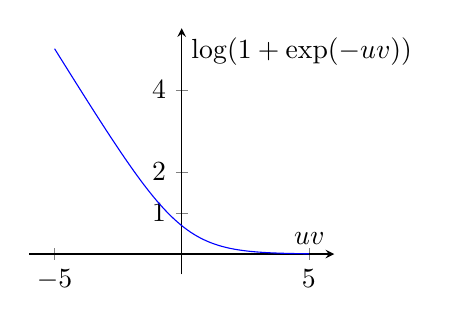
\begin{tikzpicture}
\begin{axis}[xlabel=$uv$,ylabel=$\log(1+\exp(-uv))$,ytick={1,2,4},axis lines=middle,enlargelimits,width=0.45\textwidth]
\addplot[samples=200,blue,smooth] {ln(1+exp(-x))};
\end{axis}
\end{tikzpicture}} \quad
\subfloat[][\emph{Sigmoid function}]%
{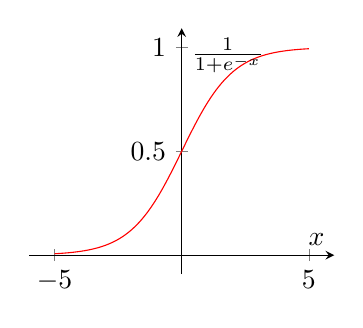
\begin{tikzpicture}
\begin{axis}[xlabel=$x$,ylabel=$\frac{1}{1+e^{-x}}$,axis lines=middle,enlargelimits,width=0.45\textwidth]
\addplot[samples=200,red,smooth] {1/(1+exp(-x))};
\end{axis}
\end{tikzpicture}}
\caption{Log-loss and sigmoid function plots}
\label{fig:log-sigma}
\end{figure}

%\begin{figure}
%	\centering
%	\subfloat[][\emph{First caption}\label{subfig:label1}]%
%	{\includegraphics[width=.45\textwidth]{}} \quad
%	\subfloat[][\emph{Second caption}\label{subfig:label2}]%
%	{\includegraphics[width=.45\textwidth]{}} \\
%	\subfloat[][\emph{Third caption}\label{subfig:label3}]%
%	{\includegraphics[width=.45\textwidth]{}} \quad
%	\subfloat[][\emph{Fourth caption}\label{subfig:label4}]%
%	{\includegraphics[width=.45\textwidth]{}} 
%	\caption[]{Global caption}
%	\label{fig:multifig}
%\end{figure}

\cleardoublepage

\begin{itemize}
\item $uv\gg0$: the example is labelled correctly
\item $uv\ll0$: the class assigned to the example is the wrong one
\end{itemize}

\begin{itemize}
\item the hessian matrix is positive defined $\forall w$, this means that the objective function, which is quadratic, is coercive and for the continuity that function admits global minimum, so $\func(w)$ has finite inferior limit
\item the hessian matrix being positive defined implies also that the objective function is strictly convex (on the other hand the loss function is just convex, due to its hessian matrix being positive semi-defined), this implies that if the global minimum exists, that solution is unique
\item a global minimum is a point that satisfy $\nabla\func(w^\ast)=0$, which is a sufficient condition implied by the convexity of the problem, see figure~\vref{subfig:log-loss}
\item the $\ell_2$ regularization implies that the objective function is strongly convex, this speeds up the convergence
\item further more we can assume that $\nabla\func(w)$ is Lipschitz-continuous with constant $L$
\end{itemize}

%\section{Theoretical results}

\cleardoublepage
\section{Mini-batch gradient descent variants}

see algorithm~\vref{code:MiniGD-fix-decr}

\subsection{Fixed step-size}

\begin{lstlisting}[style=simple,caption={Mini-batch Gradient Descent with fixed or decreasing step-size},label=code:MiniGD-fix-decr]
given £!$w^0\in\R^n$!£, £!$k=0$!£ e £!$\set{\alpha_k}\mid\alpha_k=\alpha\vee\alpha_k=\frac{\alpha_0}{k+1}$!£
while (£!$\norma{\nabla\func(w^k)}>\epsilon(1+\abs{\func(w)})$!£)
 shuffle £!$\set{1,\dots,N}$!£ and split £!$B_1,\dots,B_{N/M}$!£ such that £!$1<\abs{B_t}=M\ll N$!£
 set £!$y_0=w^k$!£
 for £!$t=1,\dots,N/M$!£
  get mini-batch indices from £!$B_t$!£
  approximate true gradient £!$\nabla f_{i_t}(w)=\frac{1}{M}\sum_{j\in B_t}\nabla f_j(y_{t-1})$!£
  compute direction £!$d_t=-\nabla f_{i_t}(y_{t-1})$!£
  make a (internal) step £!$y_t=y_{t-1}+\alpha_kd_t$!£
 end for
 update weights £!$w^{k+1}=y_{N/M}$!£
 epoch ends £!$k=k+1$!£
end while
\end{lstlisting}

%\subsection{Decreasing step-size}

\subsection{Stochastic line search}

%compute true gradient approximation £!$\nabla f_{i_t}(w)$!£ with examples from £!$B_t$!£
% define function reset()
% create function armijo_condition()
% while (£!$f_{i_t}(y_{t-1}+\alpha d_t)>f_{i_t}(y_{t-1})-\gamma\alpha\norma{\nabla f_{i_t}(y_{t-1})}^2$!£)
\begin{lstlisting}[style=simple,caption={Mini-batch Gradient Descent with Armijo line search}]
given £!$w^0\in\R^{p+1}$!£, £!$\gamma\in(0,1),\,\delta\in(0,1),\,\alpha_0\in\R^+$!£
£!$k=0$!£
while (£!$\norma{\nabla\func(w^k)}>\epsilon(1+\abs{\func(w)})$!£)
 shuffle £!$\set{1,\dots,N}$!£ and split £!$B_1,\dots,B_{N/M}$!£ such that £!$1<\abs{B_t}=M\ll N$!£
 set £!$y_0=w^k$!£
 for £!$t=1,\dots,N/M$!£
  get mini-batch indices £!$i_t$!£ from £!$B_t$!£
  approximate true gradient £!$\nabla f_{i_t}(w)=\frac{1}{M}\sum_{j\in B_t}\nabla f_j(y_{t-1})$!£
  compute direction £!$d_t=-\nabla f_{i_t}(y_{t-1})$!£
  £!$\alpha=\mathtt{reset}()$!£, £!$q=0$!£
  compute potential next step £!$y_t=y_{t-1}+\alpha d_t$!£
  while (£!$f_{i_t}(y_t)>f_{i_t}(y_{t-1})+\gamma\alpha\nabla f_{i_t}(y_{t-1})^Td_t$!£)
   reduce step-size £!$\alpha=\delta\alpha$!£
   rejections counter £!$q=q+1$!£
  end while
  set optimal mini-batch step-size £!$\alpha_t=\alpha$!£
  make a (internal) step £!$y_t=y_{t-1}+\alpha_td_t$!£
 end for
 update weights £!$w^{k+1}=y_{N/M}$!£
 epoch ends £!$k=k+1$!£
end while
\end{lstlisting}

\cleardoublepage
\subsection{Fixed momentum term}

\begin{lstlisting}[style=simple,caption={Mini-batch Gradient Descent with fixed Momentum term and fixed step-size}]
given £!$w^0\in\R^{p+1}$!£, £!$\set{\alpha_k}=\alpha$!£, £!$\set{\beta_k}=\beta\in(0,1)$!£
£!$k=0$!£
while (£!$\norma{\nabla\func(w^k)}>\epsilon(1+\abs{\func(w)})$!£)
 shuffle £!$\set{1,\dots,N}$!£ and split £!$B_1,\dots,B_{N/M}$!£ such that £!$1<\abs{B_t}=M\ll N$!£
 set £!$y_0=w^k$!£, £!$d_0=0$!£
 for £!$t=1,\dots,N/M$!£
  get mini-batch indices £!$i_t$!£ from £!$B_t$!£
  approximate true gradient £!$\nabla f_{i_t}(w)=\frac{1}{M}\sum_{j\in B_t}\nabla f_j(y_{t-1})$!£
  compute direction £!$d_t=-\bigl((1-\beta)\nabla f_{i_t}(y_{t-1})+\beta d_{t-1}\bigr)$!£
  make a (internal) step £!$y_t=y_{t-1}+\alpha_kd_t$!£
 end for
 update weights £!$w^{k+1}=y_{N/M}$!£
 epoch ends £!$k=k+1$!£
end while
\end{lstlisting}

\begin{lstlisting}[style=simple,caption={Mini-batch Gradient Descent with Armijo line search for step-size and Momentum correction}]
given £!$w^0\in\R^{p+1}$!£, £!$\gamma\in(0,1),\,\delta_a\in(0,1),\,\alpha_0\in\R^+$!£, £!$\delta_m\in(0,1),\,\beta_0\in(0,1)$!£
£!$k=0$!£
while (£!$\norma{\nabla\func(w^k)}>\epsilon(1+\abs{\func(w)})$!£)
 shuffle £!$\set{1,\dots,N}$!£ and split £!$B_1,\dots,B_{N/M}$!£ such that £!$1<\abs{B_t}=M\ll N$!£
 set £!$y_0=w^k$!£, £!$d_0=0$!£
 for £!$t=1,\dots,N/M$!£
  get mini-batch indices £!$i_t$!£ from £!$B_t$!£
  approximate true gradient £!$\nabla f_{i_t}(w)=\frac{1}{M}\sum_{j\in B_t}\nabla f_j(y_{t-1})$!£
  compute potential next direction £!$d_t=-\bigl((1-\beta)\nabla f_{i_t}(y_{t-1})+\beta d_{t-1}\bigr)$!£
  £!$q_m=0$!£
  while (£!$\nabla f_{i_t}(y_{t-1})^Td_t\geq0$!£)
   reduce momentum term £!$\beta=\delta_m\beta$!£
   rejections counter £!$q_m=q_m+1$!£
  end while
  set optimal mini-batch momentum term £!$\beta_t=\beta$!£
  £!$\alpha=\mathtt{reset()}$!£, £!$q_a=0$!£
  compute potential next step £!$y_t=y_{t-1}+\alpha d_{t-1}$!£
  while (£!$f_{i_t}(y_t)>f_{i_t}(y_{t-1})+\gamma\alpha\nabla f_{i_t}(y_{t-1})^Td_t$!£)
   reduce step-size £!$\alpha=\delta_a\alpha$!£
   rejections counter £!$q_a=q_a+1$!£
  end while
  set optimal mini-batch step-size £!$\alpha_t=\alpha$!£
  make a (internal) step £!$y_t=y_{t-1}+\alpha_td_t$!£
 end for
update weights £!$w^{k+1}=y_{N/M}$!£
epoch ends £!$k=k+1$!£
end while
\end{lstlisting}

\cleardoublepage
\begin{lstlisting}[style=simple,caption={Mini-batch Gradient Descent with Armijo line search for step-size and Momentum restart}]
given £!$w^0\in\R^{p+1}$!£, £!$\gamma\in(0,1),\,\delta_a\in(0,1),\,\alpha_0\in\R^+$!£, £!$\delta_m\in(0,1),\,\set{\beta_k}=\beta\in(0,1)$!£
£!$k=0$!£
while (£!$\norma{\nabla\func(w^k)}>\epsilon(1+\abs{\func(w)})$!£)
 shuffle £!$\set{1,\dots,N}$!£ and split £!$B_1,\dots,B_{N/M}$!£ such that £!$1<\abs{B_t}=M\ll N$!£
 set £!$y_0=w^k$!£, £!$d_0=0$!£
 for £!$t=1,\dots,N/M$!£
  get mini-batch indices £!$i_t$!£ from £!$B_t$!£
  approximate true gradient £!$\nabla f_{i_t}(w)=\frac{1}{M}\sum_{j\in B_t}\nabla f_j(y_{t-1})$!£
  compute potential next direction £!$d_t=-\bigl((1-\beta)\nabla f_{i_t}(y_{t-1})+\beta d_{t-1}\bigr)$!£
  if (£!$\nabla f_{i_t}(y_{t-1})^Td_t\geq0$!£)
   restart direction £!$d_t=d_0$!£
  end if
  £!$\alpha=\mathtt{reset()}$!£, £!$q_a=0$!£
  compute potential next step £!$y_t=y_{t-1}+\alpha d_{t-1}$!£
  while (£!$f_{i_t}(y_t)>f_{i_t}(y_{t-1})+\gamma\alpha\nabla f_{i_t}(y_{t-1})^Td_t$!£)
   reduce step-size £!$\alpha=\delta_a\alpha$!£
   rejections counter £!$q_a=q_a+1$!£
  end while
  set optimal mini-batch step-size £!$\alpha_t=\alpha$!£
  make a (internal) step £!$y_t=y_{t-1}+\alpha_td_t$!£
 end for
 update weights £!$w^{k+1}=y_{N/M}$!£
 epoch ends £!$k=k+1$!£
end while
\end{lstlisting}

%\subsection{Corrected/restart momentum}

\section{Experiments}











